\section{Minimum segment cost covers}

In this section we propose a polynomial time algorithm for solving Problem \ref{prob:min-seg-cover}.
We have seen in Chapter \ref{chapter:sr} reachability results that tells us exactly how costly,
in terms of segments, it is to deterministically reach a given node in the network. Using these results
we can easily establish how costly it is to cover a given edge with a deterministic sr-cycle.

In order to cover a given edge $e$ with a deterministic sr-cycle from $s$ to $s$ with segment cost at most
$k$, we have essentially two options:

\begin{enumerate}
 \item First we go from $s$ to some node $x$ using a deterministic sr-path of cost, say, $k_1$. Then travel
 from $x$ to some node $y$ via a unique shortest path that contains edge $e$. Finally, we go from $y$ back to $s$
 with a deterministic sr-path of cost $k_2 = k - k_1$. This is illustrated in Figure \ref{fig:cover-edge1}.
 
\begin{figure}
\begin{center}
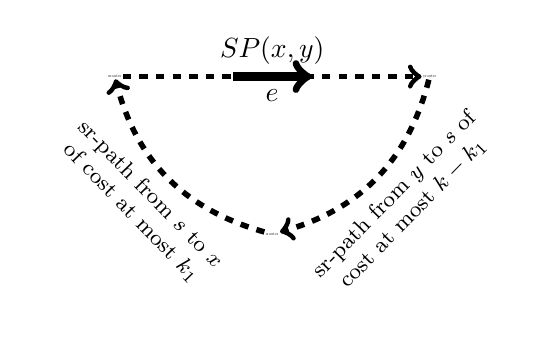
\begin{tikzpicture}
\def\x{0}
\def\y{0}

\node[scale=0.15] (s) at (0 + \x, 0 + \y)  {\router{s}{router}};
\node[scale=0.15] (x) at (-2 + \x, 2 + \y) {\router{x}{router}};
\node[scale=0.15] (y) at (2 + \x,  2 + \y) {\router{y}{router}};

\draw[line width=2, black] (s) edge[below, sloped, bend left, dashed, ->] node[black] {
\footnotesize
\begin{tabular}{c}
 sr-path from $s$ to $x$ \\
 of cost at most $k_1$
\end{tabular}
} (x);
\draw[line width=2, black] (y) edge[below, sloped, bend left, dashed, ->] node[black] {
\footnotesize
\begin{tabular}{c}
 sr-path from $y$ to $s$ of \\
 cost at most $k - k_1$
\end{tabular}
} (s);

\draw[line width=2, black] (x) edge[above, sloped, dashed, ->] node[black,font=\bfseries] {\texttt{$SP(x, y)$}} (y);

\draw[line width=3] (-0.5, 2) edge[below, ->] node {$e$} (0.5, 2);

\end{tikzpicture}
\end{center}
\caption{First case of edge covering.}
\label{fig:cover-edge1}
\end{figure}

 
 \item The second way to cover $e$ is to use an adjacency segment over it. To do so, we first go from $s$ to
 some node $x$ with a deterministic sr-path of cost at most, say, $k_1$. This node $x$ must be such that it contains 
 a unique shortest path to $e^1$. Otherwise the resulting cycle would not be deterministic. Then we use an adjacency 
 segment on $e$ to traverse it by following the unique shortest path between $x$ and $e^1$ and then $e$.
 Then we go to some node $y$ via a unique shortest path from $e^2$. Finally, we go from $y$ back to $s$ with a
 sr-path of cost at most $k_2 = k - k_1 - 2$. The $-2$ comes from the fact that we spent a segment cost of $2$ 
 with the adjacency segment $e$. This case is illustrated in Figure \ref{fig:cover-edge2}.

\begin{figure}
\begin{center}
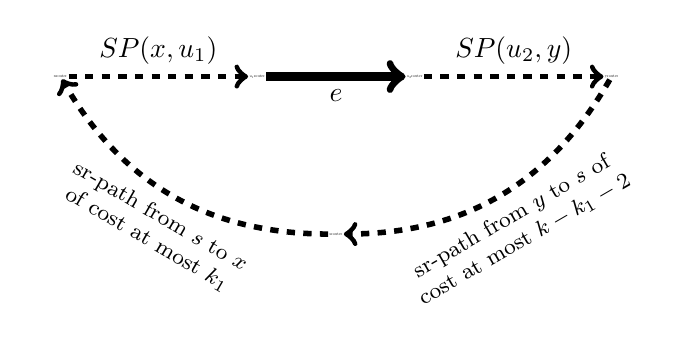
\begin{tikzpicture}
\def\x{0}
\def\y{0}

\node[scale=0.15] (s) at (0 + \x, 0 + \y)  {\router{s}{router}};
\node[scale=0.15] (x) at (-3.5 + \x, 2 + \y) {\router{x}{router}};
\node[scale=0.15] (y) at (3.5 + \x,  2 + \y) {\router{y}{router}};
\node[scale=0.15] (u1) at (-1 + \x,  2 + \y) {\router{$u_1$}{router}};
\node[scale=0.15] (u2) at (1 + \x,  2 + \y) {\router{$u_2$}{router}};

\draw[line width=2, black] (s) edge[below, sloped, bend left, dashed, ->] node[black] {
\footnotesize
\begin{tabular}{c}
 sr-path from $s$ to $x$ \\
 of cost at most $k_1$
\end{tabular}
} (x);
\draw[line width=2, black] (y) edge[below, sloped, bend left, dashed, ->] node[black] {
\footnotesize
\begin{tabular}{c}
 sr-path from $y$ to $s$ of \\
 cost at most $k - k_1 - 2$
\end{tabular}
} (s);

\draw[line width=2, black] (x) edge[above, sloped, dashed, ->] node[black,font=\bfseries] {\texttt{$SP(x, u_1)$}} (u1);
\draw[line width=2, black] (u2) edge[above, sloped, dashed, ->] node[black,font=\bfseries] {\texttt{$SP(u_2, y)$}} (y);


\draw[line width=3] (u1) edge[below, ->] node {$e$} (u2);

\end{tikzpicture}
\end{center}
\caption{Second case of edge covering.}
\label{fig:cover-edge2}
\end{figure} 
\end{enumerate}

Note that in both cases, nothings prevents us to have $x = e^1$ or $y = e^2$. We do not require these nodes to be distinct
as doing so would provide an incomplete description of all possible cases.

Next we prove formally that those two cases cover all possibilities. The next theorem directly translate into
a polynomial time algorithm for computing minimum segment cost covers.

\begin{theorem}
\label{thm:edge-cover}
Let $G$ be a network $s \in V(G)$, $e \in E(G)$ and $k \in \mathbb{N}$ an integer. There exists a deterministic sr-cycle $\sr{c}$
from $s$ to $s$ of cost at most $k$ such that $e \in E(\sr{c})$ if and only if there exist integers $k_1, k_2 \geq 1$, $x \in \nreach(k_1, s)$, $y$ such that $s \in \nreach(k_2, y)$ 
and one of the two following conditions holds
\begin{enumerate}[(1)]
 \item $k_1 + k_2 = k$, $y \in \spreach(x)$ and $e \in \sp(x, y)$
 \item $k_1 + k_2 = k - 2$, $e^1 \in \spreach(x)$ and $y \in \spreach(e^2)$
\end{enumerate}
\end{theorem}

\begin{proof}
Let $G$ be a network $s \in V(G)$, $e \in E(G)$ and $k \geq 1$ an integer.

$(\Rightarrow)$ Assume that there exists a deterministic sr-cycle $\sr{c}$ from $s$ to $s$
with $\cost(\sr{c}) \leq k$ such that $e \in E(\sr{c})$. Write $\sr{c} = \langle x_1, \ldots, x_l \rangle$.
Since $e \in E(\sr{c})$ there exists $i \in \{1, \ldots, l\}$ such that either $x_i = e$ or $i < l$ and
$e \in \sp(x^2_{i}, x^1_{i + 1})$.

\emph{Case 1:} $e \in \sp(x^2_{i}, x^1_{i + 1})$. Let $x = x^2_{i}$ and $y = x^1_{i + 1}$. Then $\sr{p} = \langle x_1, \ldots, x_{i} \rangle$ is a deterministic sr-path
from $s$ to $x$ of cost, say, $k_1$ and $\sr{q} = \langle x_{i + 1}, \ldots, x_l \rangle$ is a deterministic sr-path from $y$ to $s$ of cost $k_2 \leq k - k_1$. 
Therefore, $x \in \nreach(k_1, s)$, $s \in \nreach(k_2, y)$. Since $\sr{c}$ is deterministic, there is a unique shortest path
from $x$ to $y$ so $y \in \spreach(x)$. Since by hypothesis $e \in \sp(x, y)$, condition $(1)$ holds.

\emph{Case 2:} $e = x_i$. Let $x = x^2_{i - 1}$ and $y = x^1_{i + 1}$. Then $\sr{p} = \langle x_1, \ldots, x_{i - 1} \rangle$ is a deterministic sr-path
from $s$ to $x$ of cost, say $k_1$, and $\sr{q} = \langle x_{i + 1}, \ldots, x_l \rangle$ from $y$ to $s$ of cost, say $k_2$, such that
$k_1 + k_2 = \cost(\sr{p}) + \cost(\sr{q}) = \cost(\sr{c}) - 2 \leq k - 2$. Thus $x \in \nreach(k_1, s)$ and $s \in \nreach(k_2, y)$.
Since $\sr{c}$ is deterministic, there is a unique shortest path from $x = x^2_{i - 1}$ and $e^1 = x^1_i$. For the same reason,
there exists a unique shortest path from $e^2 = x^2_i$ to $y = x^1_{i + 1}$.  Thus $e^1 \in \nreach(2, x)$ and $y \in \spreach(e^2)$ so that
condition $(2)$ holds.

Note that in the first case we have $k_1 + k_2 \leq k$ and in the second $k_1 + k_2 \leq k - 2$ instead of the equalities. 
This is not a problem because if we have a solution with $k_1' + k_2' < k$ we also have a solution with longer paths. The same is
true for $k_1' + k_2' < k - 2$. One way to do so is to add the source $s$ enough times so that both paths have the desired segment cost.

$(\Leftarrow)$ Assume that there exist integers $k_1, k_2 \geq 1$, $x \in \nreach(k_1, s)$, $y$ such that $s \in \nreach(k_2, y)$ 
and either $(1)$ or $(2)$ holds. Since $x \in \nreach(k_1, s)$ there exists a deterministic sr-path
$\sr{p} = \langle x_1, \ldots, x_l \rangle$ from $s$ to $x$ with $\cost(\sr{p}) \leq k_1$. In the same way, since $s \in \nreach(k_2, y)$,
there exists a deterministic sr-path $\sr{q} = \langle y_1, \ldots, y_r \rangle$ from $y$ to $s$ with $\cost(\sr{q}) \leq k_2$.

\emph{Case 1:} Condition $(1)$ holds so that $k_1 + k_2 = k$, $y \in \spreach(x)$ and $e \in \sp(x, y)$. 
Let $\sr{c} = \sr{p} + \sr{q} = \langle x_1, \ldots, x_l, y_1, \ldots, y_r \rangle$. 
This sr-path is deterministic because $y^1_1 = y \in \spreach(x) = \spreach(x^2_l)$. 
For the other indexes, the unicity of shortest paths comes from the fact that both $\sr{p}$ and $\sr{q}$
are deterministic. Since $\sr{c}$ goes from $s$ to $s$ and has cost $k_1 + k_2 = k$, $\sr{c}$ is a sr-cycle of cost at most $k$ from $s$ to $s$.
It contains $e$ because $e \in \sp(x, y) = \sp(x^2_l, y^1_1)$.

\emph{Case 2:} Condition $(2)$ holds so $k_1 + k_2 = k - 2$, $e^1 \in \spreach(x)$ and $y \in \spreach(e^2)$. Let $\sr{c} = \langle x_1, \ldots, x_l, e, y_1, \ldots, y_r \rangle$.
Since $e^1 \in \spreach(x)$ and $y \in \spreach(e^2)$ we have that $\sr{c}$ is deterministic. As before, for the other indexes determinism comes from the 
determinism of $\sr{p}$ and $\sr{q}$. Finally, $\cost(\sr{c}) = \cost(\sr{p}) + \cost(\sr{q}) + \cost(e) = k_1 + k_2 + 2 \leq k - 2 + 2 = k$. Clearly $e \in \sr{c}$
so the proof is complete.
\end{proof}

Theorem \ref{thm:edge-cover} gives necessary and sufficient conditions for the existence of a sr-cycle with segment cost at most $k$
covering a given network edge. This condition is checkable in polynomial time since, if nothing better, we can just loop over all possible
candidates $x, y \in V(G)$ and splits of $k$ into $k_1, k_2$ (recall that $k \leq 2|E(G)|$).

This shows that we can solve Problem \ref{prob:min-seg-cover} in polynomial time. For each edge $e$ we compute the smallest $k$ such that
there exists a deterministic sr-cycle covering $e$. Then the maximum value over all these $k$ values will be the minimum segment cost
for which a sr-cycle cover is possible.

Algorithm \ref{algo:build-cycle} closely follows Theorem \ref{thm:edge-cover} to build a sr-cycle for a given edge $e$, source $s$ and segment cost $k$.
On lines \ref{line:case1-cycle} to \ref{line:case1-cycle-end} we try to see whether there exists $x, y, k_1$ and $k_2$ that satisfy condition $(1)$ from the 
theorem. If so, we build a cycle accordingly by putting together a deterministic sr-path from $s$ to $x$ of segment cost at most $k_1$ and a deterministic sr-path
from $y$ to $s$ of segment cost at most $k_2$. Upon failing to find such a cycle, on lines \ref{line:case2-cycle} through \ref{line:case2-cycle-end} we try to find 
$x, y, k_1$ and $k_2$ that satisfy condition $(2)$ from the theorem. If we find such values, we build a cycle composed by a deterministic sr-path from $s$ to $x$ of cost at most $k_1$,
followed by an adjacency segment on $e$ and a deterministic sr-path from $y$ to $s$ of cost at most $k_2$. If we reach line $16$ then Theorem \ref{thm:edge-cover} guarantees that
there exists no sr-cycle of segment cost at most $k$ that covers $e$ from source $s$.

\begin{algorithm}[t]
\small
\caption{$\textsf{build-srcycle}\left( G, s, k, e \right)$}
\begin{algorithmic}[1]
%\algrule
\cmtline{look for a cycle that satisfies the first set of conditions from Theorem \ref{thm:edge-cover}}
\FOR{$k_1 \in \{ 1, \ldots, k - 1\}$} \label{line:case1-cycle}
  \STATE $k_2 \gets k - k_1$
  \FOR{$x \in \nreach(k_1, s)$}
    \FOR{$y \in \spreach(x)$}
      \IF{$s \in \nreach(k_2, y)$ \textbf{and} $e \in E(\sp(x, y))$}
	\RETURN $\textsf{build-det-srpath}(G, k_1, s, x) \oplus \textsf{build-det-srpath}(G, k_2, y, s)$
      \ENDIF
    \ENDFOR
  \ENDFOR
\ENDFOR \label{line:case1-cycle-end}
\cmtline{look for a cycle that satisfies the second set of conditions from Theorem \ref{thm:edge-cover}}
\FOR{$k_1 \in \{ 1, \ldots, k - 2\}$}  \label{line:case2-cycle}
  \STATE $k_2 \gets k - k_1 - 2$
  \FOR{$x \in \nreach(k_1, s)$}
    \IF{$e^1 \in \spreach(x)$}
      \FOR{$y \in \spreach(e^2)$}
	\IF{$s \in \nreach(k_2, y)$}
	  \RETURN $\textsf{build-det-srpath}(G, k_1, s, x) \oplus \langle e \rangle \oplus \textsf{build-det-srpath}(G, k_2, y, s)$
	\ENDIF
      \ENDFOR
    \ENDIF
  \ENDFOR
\ENDFOR  \label{line:case2-cycle-end}
\RETURN \textbf{null}
\end{algorithmic}
\label{algo:build-cycle}
\end{algorithm}

By pre-computing $\nreach$ and $\spreach$ as sets with $O(1)$ membership testing, this algorithm runs in $O(k^2 \cdot |V(G)|^2 \cdot |G|)$ since the cost 
of building a path with Algorithm \ref{algo:build-det-srpath} is $O(k \cdot |G|)$. In practice thought, it will usually run much faster since the reachability sets are often quite smaller than $V(G)$ and a lot of loop iterations are cut-off beforehand by the conditions.

To check whether a cycle cover exists for a given source $s$ and segment cost $k$ we simply loop over all edges $e \in E(G)$ and check whether a cycle exists
for each of them using Algorithm \ref{algo:build-cycle}. Therefore the runtime of this algorithm is $O(k^2 \cdot |V(G)|^2 \cdot |G| \cdot |E(G)|)$. For 
completeness a formalization of this algorithm is provided as Algorithm \ref{algo:cover-exists}.

\begin{algorithm}[t]
\small
\caption{$\textsf{cover-exists}\left( G, s, k \right)$}
\begin{algorithmic}[1]
%\algrule
\FOR{$e \in E(G)$}
  \IF{$\textsf{cycle-exists}(G, s, k, e) = \textbf{null}$}
    \RETURN \textbf{false}
  \ENDIF
\ENDFOR
\RETURN \textbf{true}
\end{algorithmic}
\label{algo:cover-exists}
\end{algorithm}

To find $k$ such that a cover exists from source $s$, we perform a binary search of $k$ to find the smallest $k$ such that a cover exists. This process is described
in Algorithm \ref{algo:min-seg-cover}. Our initial search interval is $[0, 2|E(G)|]$ because we know from Lemma \ref{lemma:seg_exists}
 that any path admits a segmentation of cost at most $2 |E(G)|$.
Once we find this minimum $k$, we compute a set of sr-cycles that cover all edges. For this we iterate over all edges and compute a sr-cycle covering it with Algorithm \ref{algo:build-cycle}.
We keep a set of covered edges to which we add all edges of every new sr-cycle in the cover. In this way we reduce the total number of cycles in the final solution.
This give a total runtime of $O(\log E(G) \cdot k^2 \cdot |V(G)|^2 \cdot |G| \cdot |E(G)|)$. If the source is unknown, we can add an extra iteration over all $v \in V(G)$ to find the one 
minimizing $k$ as shown in Algorithm \ref{algo:min-seg-cover2}.


\begin{algorithm}[t]
\small
\caption{$\textsf{min-seg-cover}\left( G, s \right)$}
\begin{algorithmic}[1]
%\algrule
\cmtline{perfom a binary search to find the smallest $k$ such that a cover exists}
\STATE $lb \gets 0$
\STATE $up \gets 2|E(G)|$
\WHILE{$up - lb \geq 2$}
  \STATE $k \gets \frac{lb + up}{2}$
  \IF{$\textsf{cover-exists}\left( G, s, k \right)$}
    \STATE $up \gets k$
  \ELSE
    \STATE $lb \gets k$
  \ENDIF
\ENDWHILE
\cmtline{$k = up$ is the smallest segment cost such that a cover exists, build it}
\STATE $covered \gets \emptyset$
\STATE $C \gets \emptyset$
\FOR{$e \in E(G)$}
  \IF{$e \notin covered$}
    \STATE $\sr{c} \gets \textsf{build-srcycle}\left( G, s, ub, e \right)$
    \STATE $covered \gets covered \cup E(\sr{c})$
    \STATE $C \gets C \cup \{ \sr{c} \}$
  \ENDIF
\ENDFOR
\RETURN $C$, $ub$
\end{algorithmic}
\label{algo:min-seg-cover}
\end{algorithm}


\begin{algorithm}[t]
\small
\caption{$\textsf{min-seg-cover}\left( G \right)$}
\begin{algorithmic}[1]
%\algrule
\STATE $C^*, s^*, k^* \gets \textbf{null}, \textbf{null}, \infty$
\FOR{$s \in V(G)$}
  \STATE $C, k \gets \textsf{min-seg-cover}\left( G, s \right)$
  \IF{$k < k_min$}
    \STATE $C^*, s^*, k^* \gets C, s, k$
  \ENDIF
\ENDFOR
\RETURN $C^*$, $s^*$, $k^*$
\end{algorithmic}
\label{algo:min-seg-cover2}
\end{algorithm}


This is quite a high time complexity but it is none the less polynomial since $k \leq 2 |E(G)|$. Even tough Algorithm \ref{algo:min-seg-cover2} runs in a reasonable amount of time in practice as shown 
on Figure \ref{fig:min-seg-cover-runtime}, there is most likely a lot of space for improving it. We leave finding more efficient algorithms as an open problem on this thesis. 

\begin{algorithm}[t]
\small
\caption{$\textsf{build-det-srpath}\left( G, k, s, t \right)$}
\begin{algorithmic}[1]
%\algrule
\IF{$k = 1$}
  \RETURN $\langle s \rangle$
\ENDIF
%\cmtline{if multiple edges exist between $s$ and $t$, any will do}
\IF{$k = 2$}
  \IF{$t \in \outn(G, s)$}
    \RETURN $\langle (s, t) \rangle$ \cmt{if multiple edges exist between $s$ and $t$, any will do}
  \ENDIF
  \RETURN $\langle s, t \rangle$
\ENDIF
\FOR{$v \in \nreach(k - 1, s)$}
  \IF{$t \in \spreach(v)$}
    \RETURN $\langle t \rangle \oplus \textsf{build-det-srpath}\left( G, k - 1, s, v \right)$ 
  \ENDIF
\ENDFOR
\FOR{$v \in \nreach(k - 2, s)$}
  \FOR{$e \in \ine(G, t)$}
    \IF{$e^1 \in \spreach(v)$}
      \RETURN $\langle e \rangle \oplus \textsf{build-det-srpath}\left( G, k - 2, s, v \right)$ 
    \ENDIF
  \ENDFOR
\ENDFOR
\RETURN \textbf{null}
\end{algorithmic}
\label{algo:build-det-srpath}
\end{algorithm}

\subsubsection*{Minimum segmentation sr-cycle cover analysis}

Figure \ref{fig:min-seg-cover-runtime} shows that the maximum time taken over any topology to compute a minimum sr-cycle cover
with an unknown source was about $15$ minutes. This is a reasonable amount of time given that network monitoring covers are often
computed only once and only need to change when the topology changes. A $15$ minute setup time for a link failure monitoring service
seems perfectly usable in practice.

\begin{figure}
\begin{center}
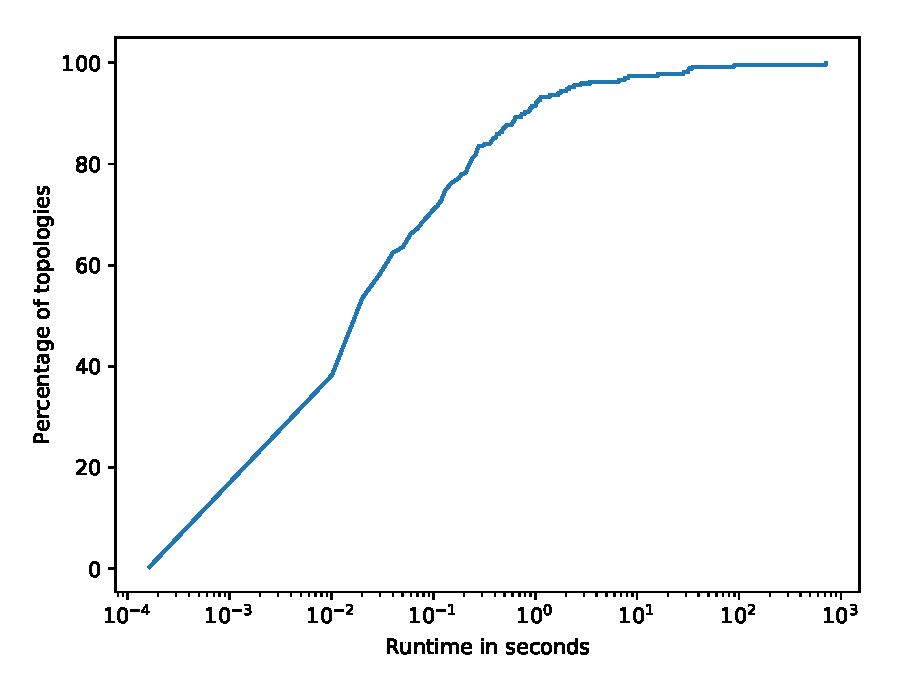
\includegraphics[width=.85\columnwidth]{./Network-lib/data/plot/minSegCover_runtime.eps}
\end{center}
\caption{Runtime CDF of Algorithm \ref{algo:min-seg-cover2} over all topologies.}
\label{fig:min-seg-cover-runtime}
\end{figure}

Figure \ref{fig:min-seg-cover-runtime-size} shows the runtime of ref{algo:min-seg-cover2} with respect to
the size of the topology $|G|$. We can observe that it indeed performs much better in practice than its theoretical
time complexity.

\begin{figure}
\begin{center}
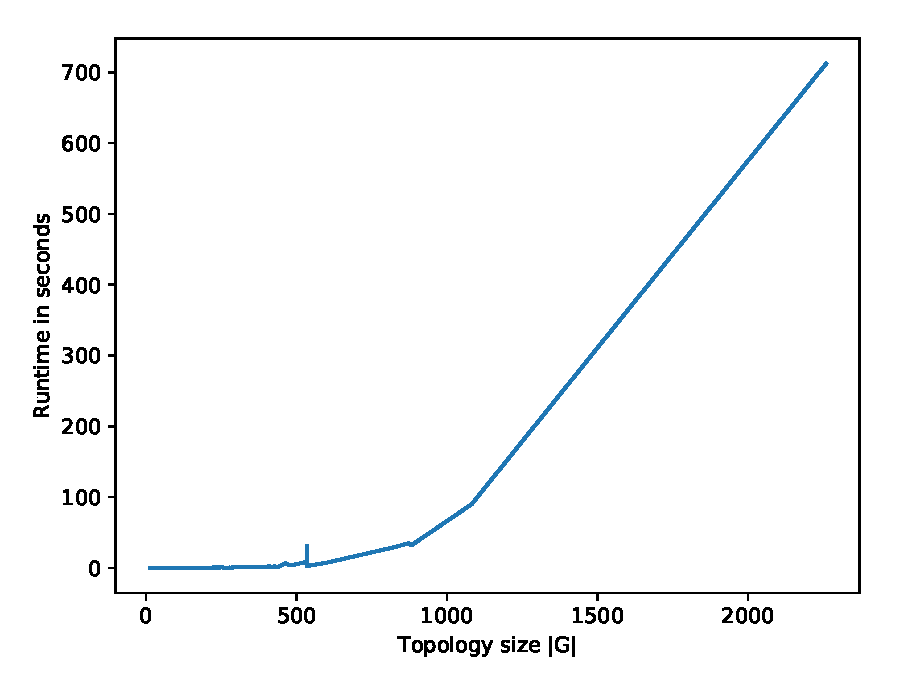
\includegraphics[width=.85\columnwidth]{./Network-lib/data/plot/minSegCover_runtime_by_size.eps}
\end{center}
\caption{Runtime by topology size of Algorithm \ref{algo:min-seg-cover2} over all topologies.}
\label{fig:min-seg-cover-runtime-size}
\end{figure}

Next, we analyze the segment cost of the sr-cycle covers produced by the algorithm. This gives a lower bound
on the segment cost of \emph{any} cycle cover on the given topologies. This is an important result as it shows
whether or not we can expect to be able to implement such a monitoring scheme on a segment routed network. As
we can see on Figure \ref{fig:min-seg-cover-segcost}, for more than $70\%$ we can find a cycle cover needing
at most a segment cost of $5$. This means that in most topologies such a sr-cycle cover is implementable even
on a network operating low end routers. Almost all topologies require a segment cost of at most $10$ showing
that network monitoring with segment routing is realistic for most topologies with high end routers. We wanted
to analyze the relationship between the size of the topology and the segment cost required for the sr-cycle cover.
The is shown in Figure \ref{fig:min-seg-cover-segcost-size}. We can see that the size does not seem to be 
correlated with the minimum segment cost.

\begin{figure}
\begin{center}
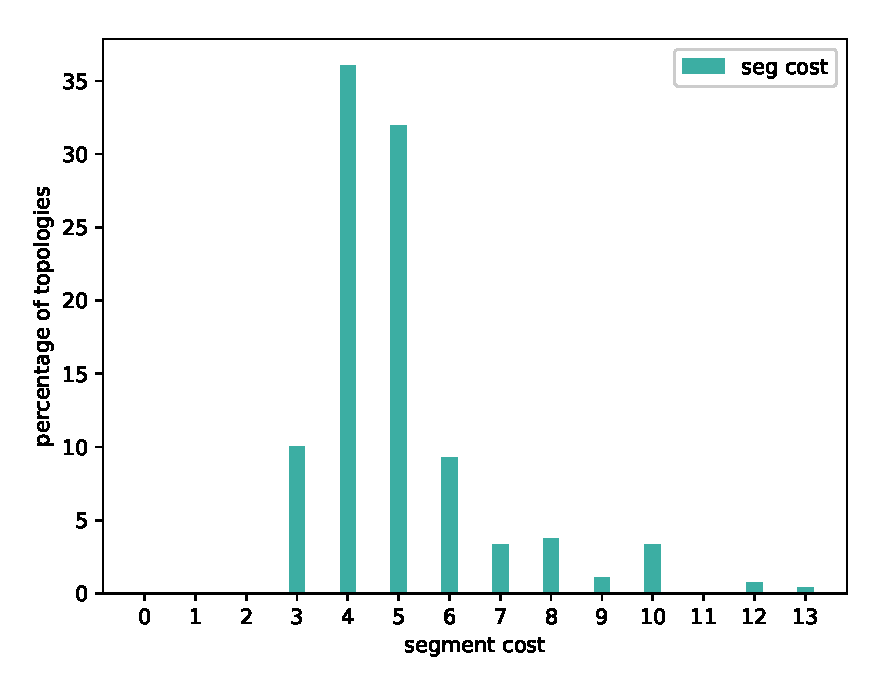
\includegraphics[width=.85\columnwidth]{./Network-lib/data/plot/minSegCover_segcost.eps}
\end{center}
\caption{Percentage of topologies for each segment cost.}
\label{fig:min-seg-cover-segcost}
\end{figure}


\begin{figure}
\begin{center}
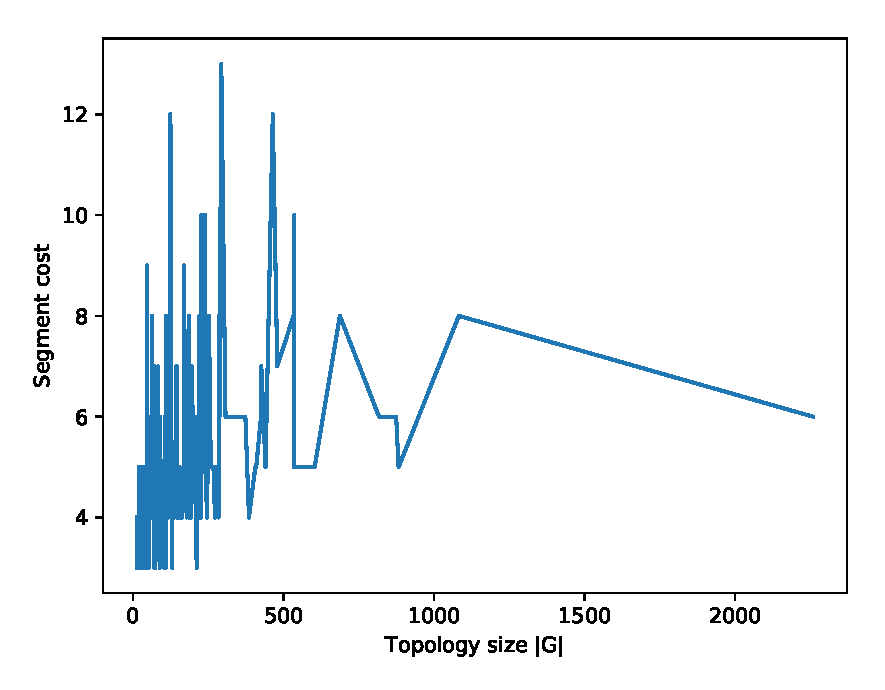
\includegraphics[width=.85\columnwidth]{./Network-lib/data/plot/minSegCover_segcost_by_size.eps}
\end{center}
\caption{Segment cost by topology size over all topologies.}
\label{fig:min-seg-cover-segcost-size}
\end{figure}
